\receta{Habichuelas con Carne}


\begin{ingredientes}
\item 500g Habichuelas Picada
\item 500g Carne de res
\item 250g Pasta de tomate
\item 40g Aceite
\item Agua
\item Sal
\item Pimienta Dulce
\item Pimienta Negra
\end{ingredientes}
\preparacion

Hierva en una olla las habichuelas picadas en cuadritos y resérvelas con el agua. Sofría la carne con el aceite, y posteriormente agregue la pasta de tomate. Cuando  la pasta se torne obscura, agregue las habichuelas con el agua para formar salsa, dejando reducir a fuego medio. Finalmente, cuando la consistencia de la salsa sea espesa, se adoba la mezcla con las pimientas y la sal.\\

\clearpage
\vspace*{5cm}
\begin{center}
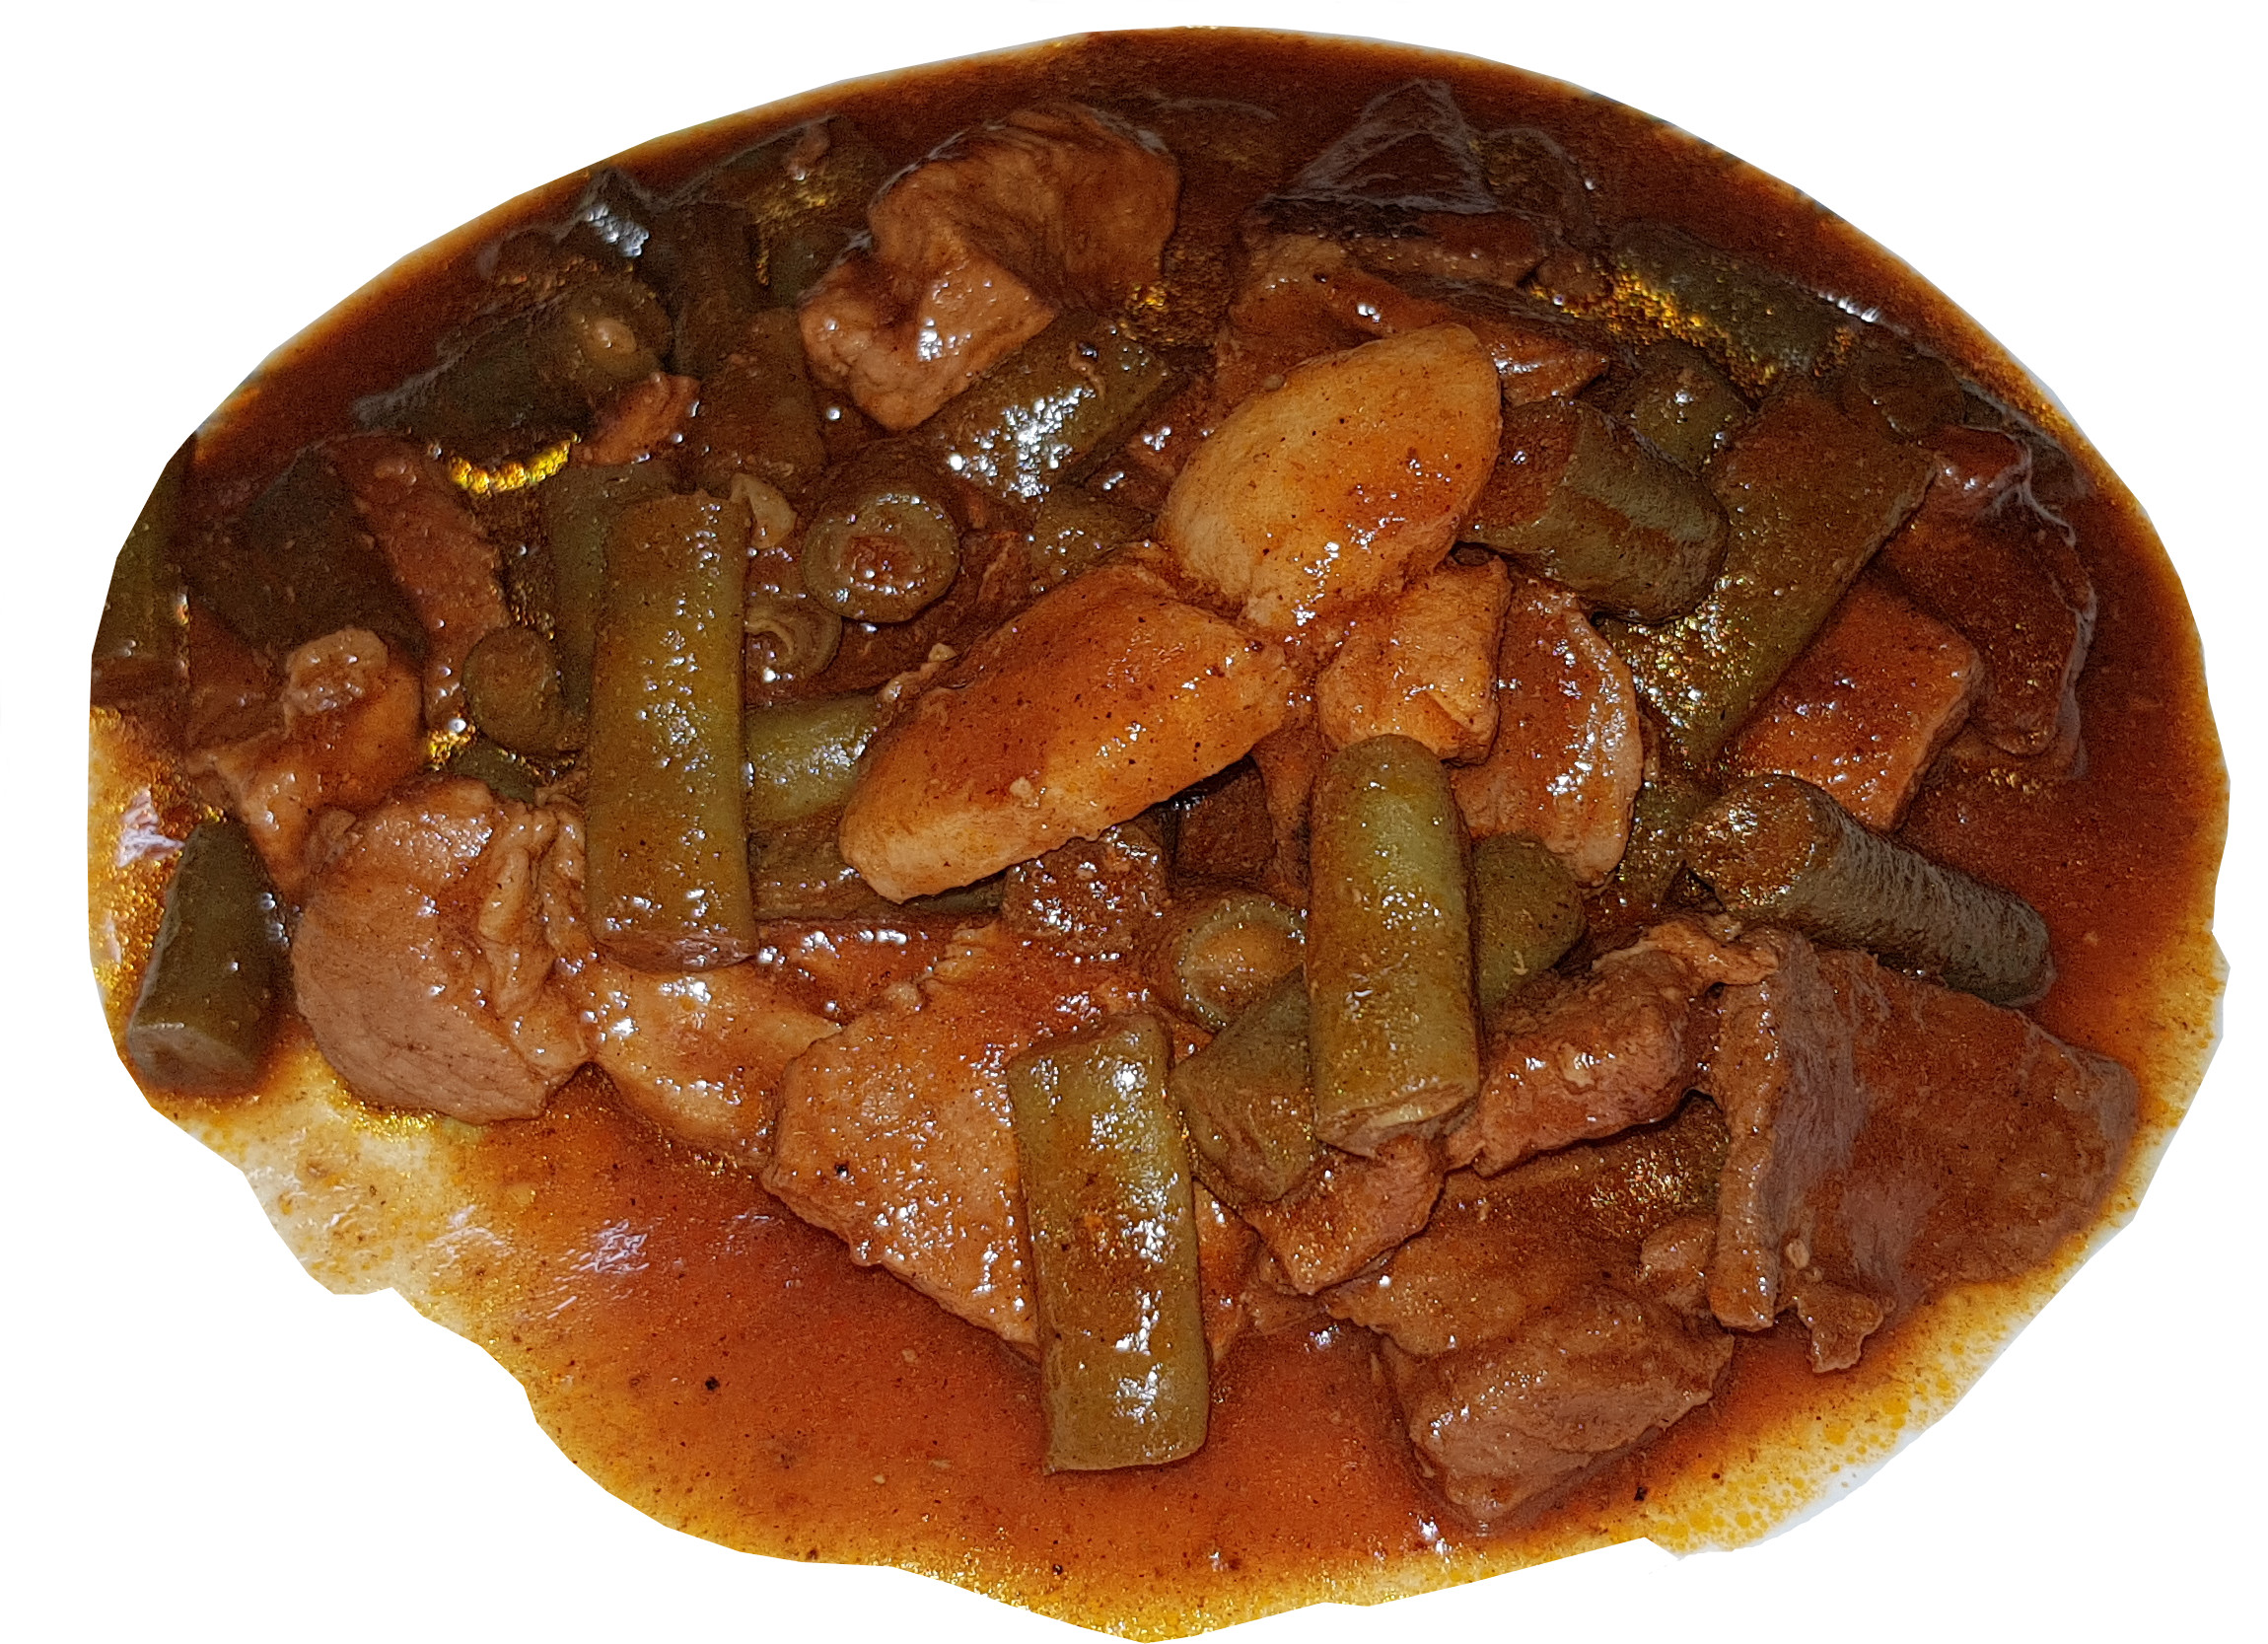
\includegraphics[width=\textwidth]{fotos/habichuelas.jpg} 
\end{center}


